
\documentclass[border=1pt]{standalone}
\usepackage[T1]{fontenc}
\usepackage{newtxtext}
\usepackage{newtxmath}
\usepackage{amsmath}
\usepackage{tikz}
\usepackage{pgfplots}
\usepgfplotslibrary{groupplots}
\usetikzlibrary{arrows.meta}
\pgfplotsset{compat=1.18}

\definecolor{cclassical}{HTML}{2166ac}
\definecolor{clearned}{HTML}{b2182b}
\definecolor{cproposed}{HTML}{1a9850}
\definecolor{cref}{HTML}{7f7f7f}
\definecolor{clight}{HTML}{67a9cf}
\definecolor{cbandlo}{HTML}{f4a582}
\definecolor{cbandhi}{HTML}{92c5de}

% Figure text is sized for a 252 pt column: axis labels a touch under the
% 8 pt caption size, tick labels one step below that.
\newcommand{\figlab}{\fontsize{7.5}{8.5}\selectfont}
\newcommand{\figtick}{\fontsize{6.5}{7.5}\selectfont}
\newcommand{\fignote}{\fontsize{6}{7}\selectfont}

\pgfplotsset{
  every axis/.append style={
    line width=0.5pt,
    scale only axis,
    tick style={line width=0.4pt, black},
    tick pos=left,
    grid=major,
    grid style={gray!30, line width=0.3pt},
    label style={font=\figlab},
    tick label style={font=\figtick},
    title style={font=\figlab, yshift=-2pt},
    legend cell align=left,
    legend style={
      font=\fignote, draw=black!35, fill=white, fill opacity=0.92,
      text opacity=1, inner sep=1.2pt, row sep=-1.5pt, legend image post style={scale=0.7}},
  },
  every axis plot/.append style={line width=0.7pt, mark size=1.3pt},
}
\begin{document}
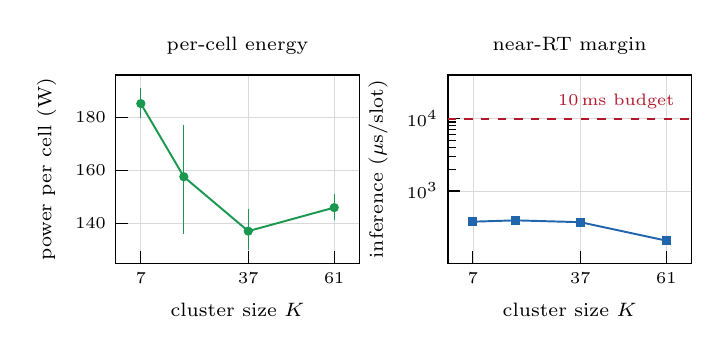
\begin{tikzpicture}
\begin{groupplot}[
  group style={group size=2 by 1, horizontal sep=32pt},
  width=88pt, height=68pt, xlabel={cluster size $K$},
]
\nextgroupplot[title={per-cell energy}, ylabel={power per cell (W)}, xmin=0, xmax=68, xtick={7,37,61}]
\addplot[cproposed, mark=*, error bars/.cd, y dir=both, y explicit,
  error bar style={line width=0.4pt}, error mark options={line width=0.4pt, mark size=1pt}]
  table[x=x, y=y, y error plus=ep, y error minus=em] {
x y ep em
7 185.19 4.84421 4.45889
19 157.564 18.6644 20.5073
37 137.042 7.46145 6.21767
61 145.932 3.9313 3.8135
};

\nextgroupplot[title={near-RT margin}, ymode=log, ylabel={inference ($\mu$s/slot)}, xmin=0, xmax=68, xtick={7,37,61}, ymin=100, ymax=40000, ytick={1e3,1e4}]
\addplot[cclassical, mark=square*] coordinates {(7,376.039) (19,392.271) (37,370.031) (61,205.572)};
\addplot[clearned, dashed, forget plot] coordinates {(0,10000) (68,10000)};
\node[font=\fignote, text=clearned, anchor=south east] at (axis cs:66,10000) {10\,ms budget};
\end{groupplot}
\end{tikzpicture}
\end{document}
